\documentclass{template/template}

\usepackage{subcaption}
\usepackage{amsmath}
\usepackage{enumitem}
\usepackage{hyperref}
\usepackage{gensymb} % balíček symbolů
\usepackage{booktabs}

\usepackage[toc,page]{appendix}
\usepackage{color} % balíček pro obarvování textů
\usepackage{xcolor}  % zapne možnost používání barev, mj. pro \definecolor
\definecolor{mygreen}{RGB}{0,150,0} % nastavení barev odkazů 
\usepackage{listings} % balíček pro formátování zdrojových kódů 
\usepackage[author=,status=draft]{fixme} % vkládání poznámek  
% dva módy (status): draft (poznámky se zobrazují v PDF) / final (poznámky se nezobrazují v PDF)
\usepackage{multirow}
\usepackage{float}

\lstset { %
    language=C++,
    backgroundcolor=\color{black!5}, % set backgroundcolor
    basicstyle=\footnotesize,% basic font setting
}

\addbibresource{text.bib}
\nocite{*}

\titlecz{Využití videonávodů pro výuku konstrukce v SolidWorks} % Název práce
\titleen{Videoguides usage in SolidWorks construction education} % Anglický název práce
\author{Petr Štourač} % Jméno autora
\institution{STŘEDNÍ PRŮMYSLOVÁ A VYŠŠÍ ODBORNÁ ŠKOLA BRNO, Sokolská} % Celý název instituce
\institutiontype{příspěvková organizace} % Typ instituce
\thesistype{Maturitní práce}  % Typ práce/dokumentu
\mentor{Ing. Václav Zavadil} % Jméno vedoucího práce
\mentorstatement{Ing. Václava Zavadila} % Jméno vedoucího práce ve čtvrtém pádě
\field{Strojírenská konstrukce} % Okruh, nebo téma

\placefooter{Brno 2021}

%\usepackage{hyperref} % balíček pro hypertextové odkazy
% \url{www.odkaz.cz}
% \href{http://www.odkaz.cz}{Text který bude jako odkaz}
% \hyperlink{label}{proklikávací_text} - odkaz na text 
% \hypertarget{label}{cíl_odkazu} - cíl odkazu 

\begin{document}

\maketitle

\makecopyrightstatement{V~Brně}

\makethanks{Duis ante orci, molestie vitae vehicula venenatis, tincidunt ac pede. Nemo enim ipsam voluptatem quia voluptas sit aspernatur aut odit aut fugit, sed quia consequuntur magni dolores eos qui ratione voluptatem sequi nesciunt. Proin pede metus, vulputate nec, fermentum fringilla, vehicula vitae, justo. Pellentesque arcu. Cum sociis natoque penatibus et magnis dis parturient montes, nascetur ridiculus mus. Fusce aliquam vestibulum ipsum. Aenean placerat. Excepteur sint occaecat cupidatat non proident, sunt in culpa qui officia deserunt mollit anim id est laborum. Vivamus porttitor turpis ac leo. Nullam eget nisl. Maecenas libero. Nunc auctor. Nullam rhoncus aliquam metus. Integer pellentesque quam vel velit.}

\pagestyle{empty}

\section*{Anotace}
Sem patří anotace v češtině.

\subsection*{Klíčová slova}
5 a příp. více klíčových slov

\vspace{20mm}

\section*{Annotation}
Here goes english version of thesis annotation.
\fxnote[author=PŠ]{Nějak takto vypadá poznámka vytvořená přes fxnote}

\fxnote[author=PŠ]{\textcolor{mygreen}{A dokonce je lze obarvit!}}

\subsection*{Keywords}
Here goes 5 or more keywords

\newpage
\pagestyle{plain}

\tableofcontents % vysází obsah

%%% Začátek práce
\setcounter{figure}{0}
\setcounter{table}{0}
\newpage

% Uvod prace
\chapter*{Úvod}
\addcontentsline{toc}{chapter}{Úvod}
Sem přijde úvod práce.

\newpage


% Uspory dosazene pouzitim protoplantu
\chapter{Kapitola --}


\newpage

% Zaver prace
\chapter*{Závěr}
\addcontentsline{toc}{chapter}{Závěr}
Sem přijde závěr práce.

\newpage
\newpage

\appendix
\addcontentsline{toc}{chapter}{Přílohy}

% Prilohy
\chapter{Obrazové přílohy}

\begin{figure}[h]
    \centering
    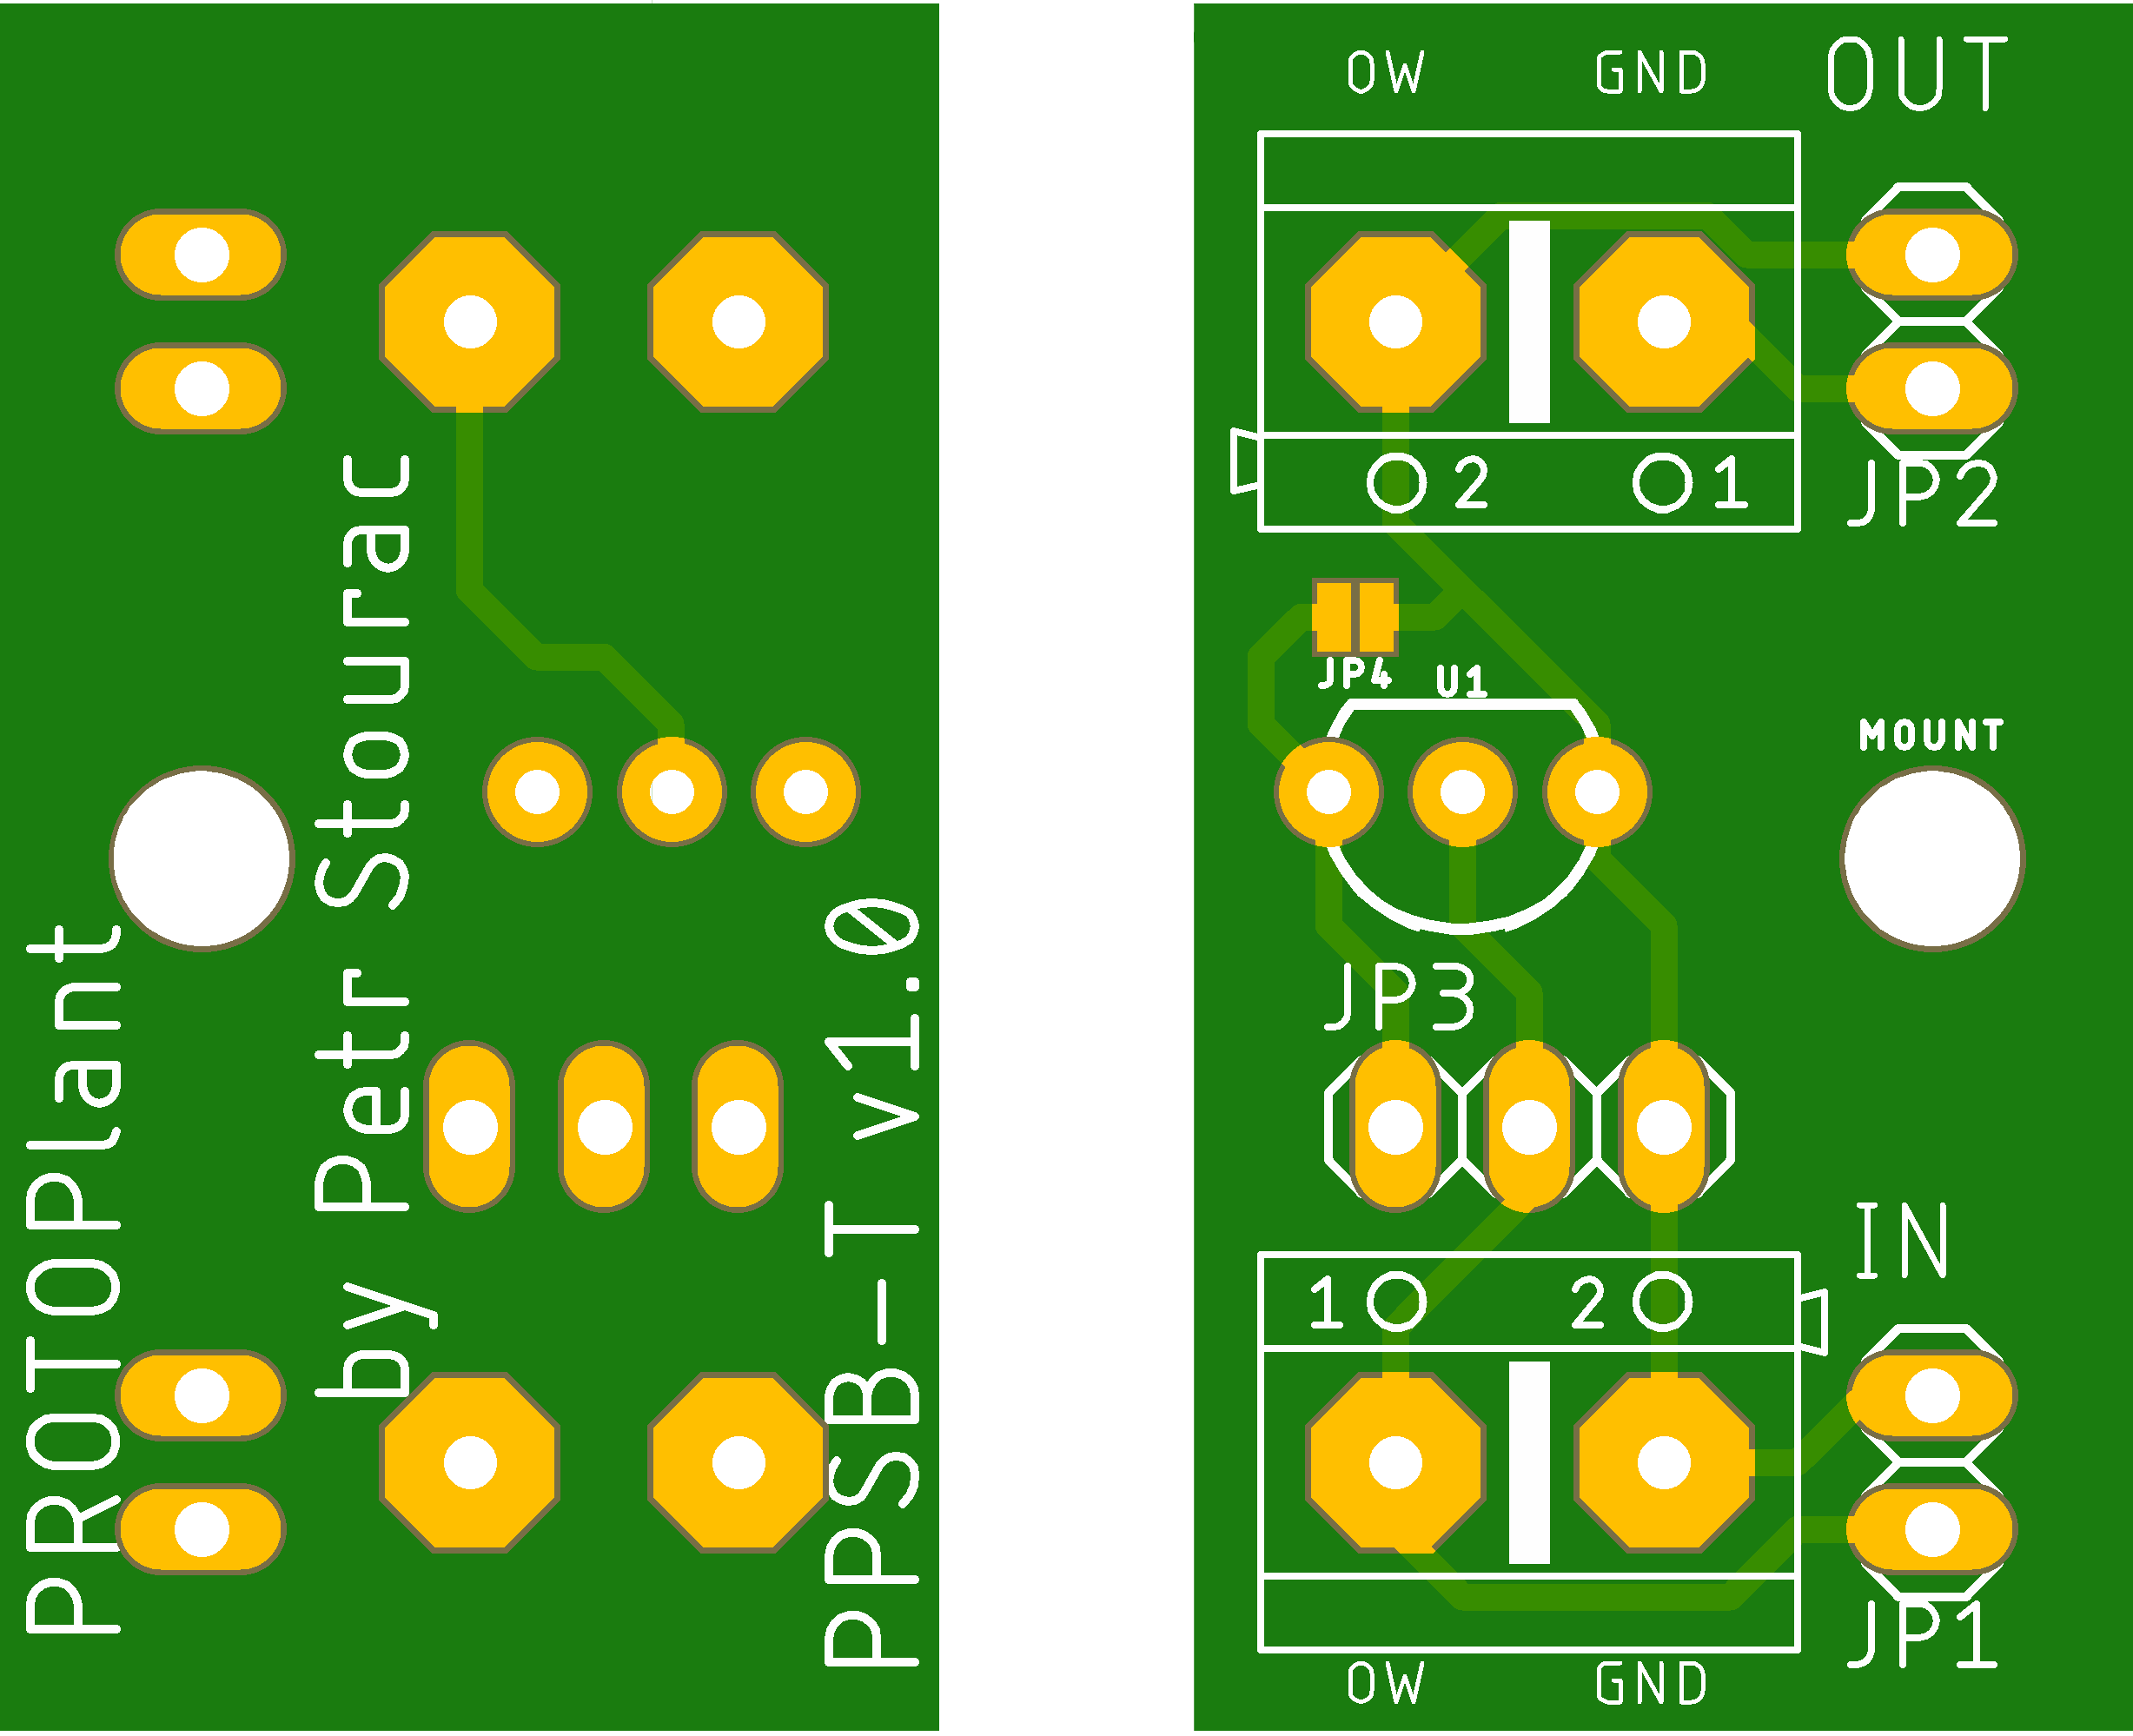
\includegraphics[width=0.85\textwidth]{img/ToBeRemoved/PPSB-T_BOTH.png}
    \caption{Vizualizace PPSB-T (horní strana vpravo, dolní vlevo).}
    \label{fig:PPSB-T_VISUAL}
\end{figure}

\printbibliography[title=Literatura]
\addcontentsline{toc}{chapter}{Literatura}

\listoffigures
\addcontentsline{toc}{section}{Seznam obrázků}

\listoftables
\addcontentsline{toc}{section}{Seznam tabulek}

\end{document}
